\documentclass[12pt]{article}

\usepackage{hcmus-report-template}
\usepackage{graphicx}
\usepackage{subfigure}
\usepackage{hyperref}

% Disable indentation on new paragraphs
\setlength{\parindent}{0pt}

% Line spacing 1.5
\renewcommand{\baselinestretch}{1.5}

% Optional: graphic path
% \graphicspath{PATH_TO_GRAPHIC_FOLDER}

% To use Times font family, uncomment this row
% \usepackage{mathptmx}

% To use roman section / subsection, uncomment these rows
% \renewcommand{\thesection}{\Roman{section}}
% \renewcommand{\thesubsection}{\thesection.\Roman{subsection}}

% Define course name, report name and report title.
\newcommand{\coursename}{Xử lý ảnh và video số}
\newcommand{\reportname}{THỰC HÀNH VỚI YOLO}
\newcommand{\reporttitle}{Báo cáo bài thực hành 4}

\newcommand{\studentname}{Lê Châu Hữu Thọ (22120350)}
\newcommand{\teachername}{Thầy Lý Quốc Ngọc \\Thầy Phạm Minh Hoàng\\Thầy Nguyễn Mạnh Hùng\\Thầy Phạm Thanh Tùng}

% Header
\lhead{\reporttitle}
\rhead{
Trường Đại học Khoa học Tự nhiên - ĐHQG HCM\\
\coursename
}



% ============ DOCUMENT ============
\begin{document}

\pagenumbering{roman}
\begin{titlepage}
\newcommand{\HRule}{\rule{\linewidth}{0.5mm}}
\centering

\textsc{\LARGE đại học quốc gia tphcm}\\[0.5cm]
\textsc{\Large trường đại học khoa học tự nhiên}\\[0.5cm]
\textsc{\large khoa công nghệ thông tin}\\[0.5cm]
\textsc{bộ môn khoa học máy tính}\\[0.5cm]

\HRule \\[0.4cm]
{ 
\huge{\bfseries{\reporttitle}}\\[0.5cm]
\large{\bfseries{Đề tài: \reportname}}
}\\[0.4cm]
\HRule \\[0.5cm]

\textbf{\large Môn học: \coursename}\\[0.5cm]

\begin{minipage}[t]{0.4\textwidth}
\begin{flushleft} \large
\emph{Sinh viên thực hiện:}\\
\studentname
\end{flushleft}
\end{minipage}
~
\begin{minipage}[t]{0.4\textwidth}
\begin{flushright} \large
\emph{Giáo viên hướng dẫn:} \\
\teachername
\end{flushright}
\end{minipage}\\[1cm]

{\large \today}\\[1cm]


\includegraphics[scale=.20]{img/hcmus-logo.png}\\[1cm] 

\vfill
\end{titlepage}
	

\tableofcontents
\pagebreak
\listoftables
\pagebreak
\listoffigures
\pagebreak

\pagenumbering{arabic}
\setcounter{page}{1}

\section{Tự đánh giá}

\subsection{Bảng đánh giá}
 
 \begin{table}[H]
     \centering
     \begin{tabular}{|l|c|} \hline 
          Viết mã nguồn đầy đủ& 100\%\\ \hline 
          Viết báo cáo đầy đủ& 100\%\\ \hline 
          Thu thập và xử lí dữ liệu & 100\%\\ \hline
          Huấn luyện mô hình & 100\%\\ \hline
          Xuất ảnh minh họa dự đoán sau huấn luyện & 100\%\\ \hline
     \end{tabular}
     \caption{Tự đánh giá công việc}
     \label{tab:my_label}
 \end{table}

\subsection{Các nội dung chưa hoàn thành}
\begin{itemize}
    \item Bài tập điểm cộng
\end{itemize}

\section{Giới thiệu}
\subsection{Giới thiệu mô hình}
Mô hình được sử dụng trong bài thực hành là \textbf{YOLOv10}, đây là phiên bản \textbf{YOLO} được phát hình vào tháng 5/2024. Lí do sử dụng mô hình \textbf{YOLOv10} thay cho \textbf{YOLOv4} là do sự tương thích của \textbf{YOLOv10} với phiên bản hiện tại của Colab là 3.10.12 (so với \textbf{YOLOv4} là 3.6/3.7). Đồng thời tránh việc xung đột giữa các thư viện được yêu cầu cài đặt so với các thư viện hiện có trong Colab.

\subsection{Đánh giá hiệu suất mô hình}

\begin{figure}[H]
    \centering
    \subfigure[ ]{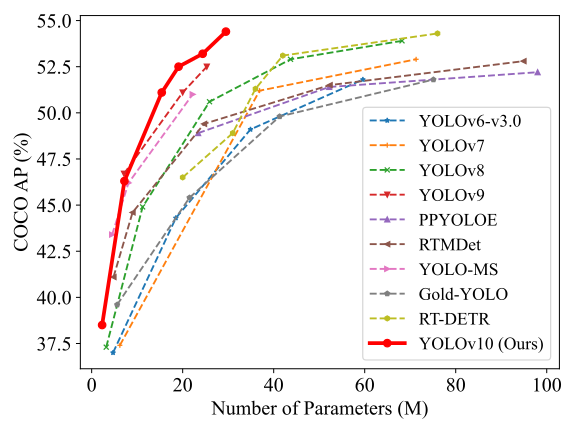
\includegraphics[scale=0.4]{img/params.png}}
    \quad % Khoảng cách ngang giữa các ảnh
    \subfigure[ ]{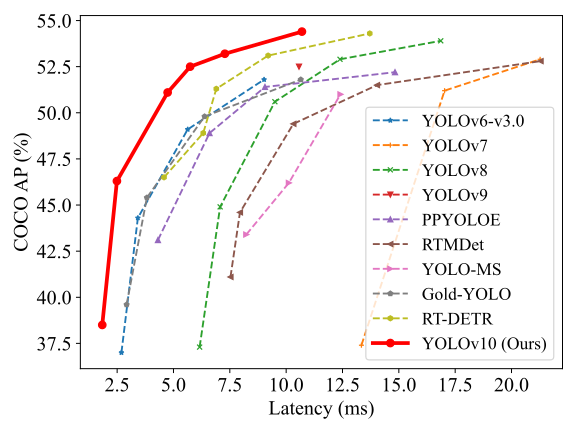
\includegraphics[scale=0.4]{img/latency.png}}
    \caption{Đánh giá hiệu suất các mô hình theo độ trễ (Latency) và số tham số (Parameters)}
    \label{fig:multiple_images}
\end{figure}

Các mô hình được đánh giá trên tập dữ liệu COCO. Về số lượng tham số, YOLOv10 cho thấy độ chính xác cao nhất ở mức tham số nhỏ và vừa. Đồng thời ở giá trị độ trễ, YOLOv10 cũng cho độ chính xác tốt nhất ở các mức độ trễ thấp nhất. Điều này cho thấy YOLOv10 đã cải thiện đáng kể về cả độ chính xác, hiệu năng và tốc độ xử lí so với các mô hình tiền nhiệm. 
\section{Bộ dữ liệu}
\subsection{Giới thiệu}
Bộ dữ liệu được sử dụng trong bài thực hành là bộ dữ liệu về đồ nội thất. Bộ dữ liệu được sử dụng để huấn luyện các mô hình xác định một số loại vật liệu nội thất phổ biến từ trong ảnh.
\subsection{Mô tả dữ liệu}
\begin{itemize}
    \item \textbf{Tác giả}: \href{https://universe.roboflow.com/minoj-selvaraj/}{Minoj Selvaraj}
    \item \textbf{Chứng chỉ}: \href{https://creativecommons.org/licenses/by/4.0/}{CC BY 4.0}
    \item \textbf{Tổng số dữ liệu}: 689
    \item \textbf{Phân bổ dữ liệu theo tập train/valid/test:}
    \begin{itemize}
        \item \textbf{Train}: 454
        \item \textbf{Valid}: 161
        \item \textbf{Test}: 74
    \end{itemize}
    \item \textbf{Số lớp nhãn dán}: 3: Chair, Sofa, Table
    \item \textbf{Định dạng}: tương thích với mô hình YOLOv7 trở lên 
    \item \textbf{Dữ liệu không có nhãn}: 0
\end{itemize}


\section{Hướng dẫn cài đặt và huấn luyện mô hình bằng Google Colab}
\subsection{Kiểm tra môi trường}
Trong giao diện chính của Colab, chọn mục \textbf{Runtime} $\xrightarrow{}$ \textbf{Change runtime type} $\xrightarrow{}$ \textbf{T4 GPU} để chuyển sang chế độ GPU
\begin{figure}[H]
\centering
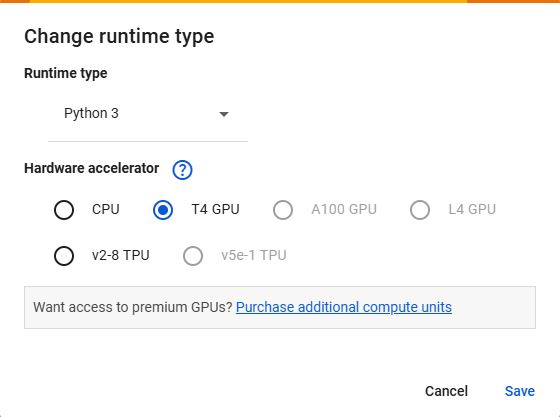
\includegraphics[scale=.4]{img/gpu.JPG}
\caption{Chuyển sang chế độ GPU}
\label{fig:my_label_with_H}
\end{figure}

Có thể kiểm tra lại thông tin GPU bằng câu lệnh
\begin{lstlisting}[language=tex]
!nvidia-smi
\end{lstlisting}

\subsection{Cấp quyền cho Drive}
Cấp quyền để Colab truy cập vào thư mục Drive của người dùng thông qua đoạn mã sau:
\lstinputlisting[language=Python]{code/drive.py}

\subsection{Tải tập tin pretrain}
Tập tin pretrain dùng trong mô hình huấn luyện. Người dùng chỉ cần chọn tập tin pretrain thích hợp và huấn luyện tiếp bộ trọng số có trong tập tin đó để tiết kiệm thời gian thay vì phải huấn luyện mô hình từ con số 0. YOLOv10 cung cấp nhiều tập tin pretrain khác nhau tùy theo mục đích người sử dụng. Dưới đây là đoạn mã ví dụ tải tập tin pretain YOLOv10 - N:
\lstinputlisting[language=Python]{code/pretrain.py}

\subsection{Cài đặt bộ dữ liệu}
\subsubsection{Định dạng cây thư mục dữ liệu}
Đối với các thư mục dữ liệu được sử dụng cho mô hình YOLOv7 trở lên, cây thư mục cần phải có định dạng như sau:
\lstinputlisting[language=tex]{code/tree.tex}
\subsubsection{Cáu trúc tập tin .yaml}
Trong các mô hình YOLOv7 trở lại đây, tập tin .yaml là một tập tin có chức năng hướng dẫn mô hình cần phải trỏ tới thư mục nào để lấy dữ liệu dùng để huấn luyện, đồng thời xác định các lớp nhãn dán có trong mô hình. Cấu trúc một tập tin .yaml gồm có các thành phần như sau:
\begin{itemize}
    \item \textbf{train:} Đường dẫn đến thư mục chứa ảnh trong tập train. Ví dụ: /train/images
    \item \textbf{valid:} Đường dẫn đến thư mục chứa ảnh trong tập valid. Ví dụ: /valid/images
    \item \textbf{train:} Đường dẫn đến thư mục chứa ảnh trong tập test. Ví dụ: /test/images
    \item \textbf{nc:} số lớp nhãn dán
    \item \textbf{names:} danh sách tên các lớp nhãn dán.
\end{itemize}
\subsubsection{Cấu trúc tập tin nhãn dán}
Nội dung của một file nhãn dán trong bộ dữ liệu có thể gồm một số dòng nhất định, trong đó mỗi dòng tượng trưng cho nhãn dán của một đối tượng. Nội dung nhãn dán của một đối tượng có cấu trúc như sau
\begin{lstlisting}[language=tex]
<class_id> <x_center> <y_center> <width> <height>
\end{lstlisting}
Trong đó:
\begin{itemize}
    \item \textbf{class\_id}: ID của lớp đối tượng, là giá trị nguyên bắt đầu từ số 0, phải khớp với thứ tự trong danh sách \textbf{names} trong file .yaml
    \item \textbf{x\_center}: Tọa độ tâm của đối tượng theo chiều ngang.
    \item \textbf{y\_center}: Tọa độ tâm của đối tượng theo chiều dọc.
    \item \textbf{width}: Độ rộng của bounding box.
    \item \textbf{height}: Độ cao của bounding box.
\end{itemize}

Lưu ý: Tên tập tin nhãn dán phải khớp với tên tập tin ảnh. Ngoại trừ \textbf{class\_id}, các giá trị khác của đối tượng phải được chuẩn hóa về khoảng (0, 1) theo tỉ lệ độ dài/rộng của ảnh.

Ví dụ: Một ảnh có kích thước rộng/dài là 800x600 và có thông tin đối tượng như sau:
\begin{itemize}
    \item ID: 0
    \item Tọa độ chưa được chuẩn hóa: (400, 300, 200, 150)
    \item Chuẩn hóa tọa độ tâm: x\_center = 400/800 = 0.5, y\_center = 300/600 = 0.5
    \item Chuẩn hóa kích thước hộp: width = 200/800 = 0.25, height = 150/600 = 0.25
    \item Nhãn dán đã chuẩn hóa: (0, 0.5, 0.5, 0.25, 0.25)
\end{itemize}

\subsection{Huấn luyện mô hình}
Để huấn luyện mô hình, ta chỉ cần gọi thư viện YOLOv10 đẫ tải về trước đó, sau đó gọi lệnh \textbf{!yolo} kèm với đường dẫn chứa tập tin pretrain, tập tin .yaml và một số thông số khác. Dưới đây là ví dụ về đoạn mã huấn luyện mô hình:

\lstinputlisting[language=Python]{code/train.py}

Nếu mô hình được cài đặt và huấn luyện thành công, kết quả trả về sẽ như trong hình minh họa dưới đây.

\begin{figure}[H]
\centering
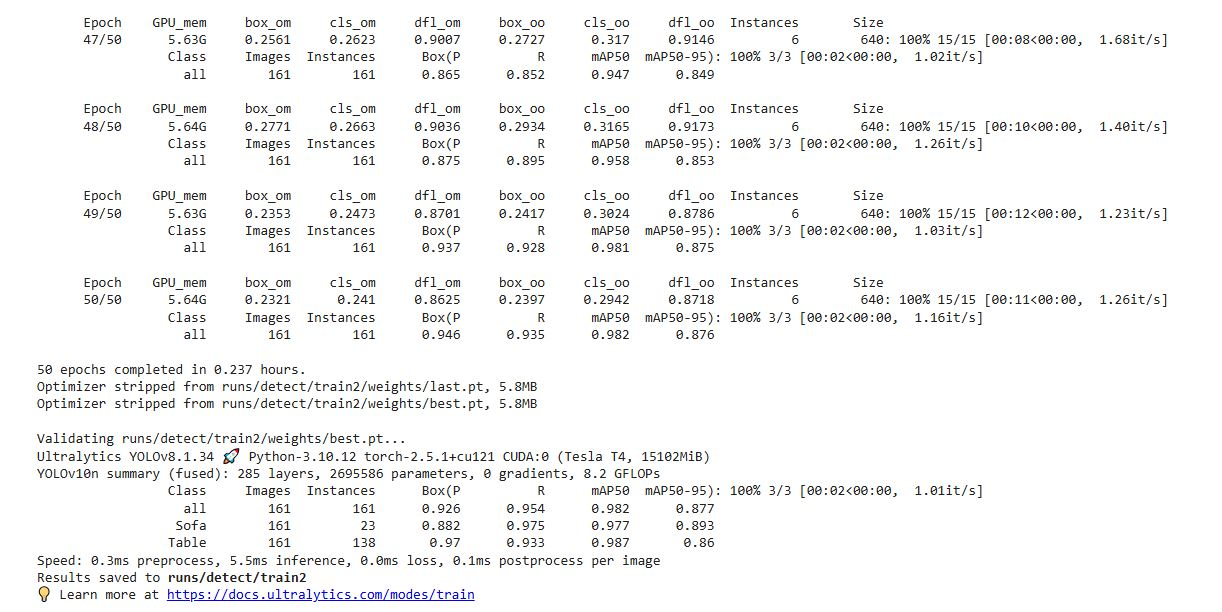
\includegraphics[scale=.5]{img/train.JPG}
\caption{Kết quả sau khi huấn luyện}
\label{fig:my_label_with_H}
\end{figure}
\section{Đánh giá mô hình}
\subsection{Thông số huấn luyện}
Mô hình được huấn luyện với các thông số như sau:
\begin{itemize}
    \item Tập tin pretrain: YOLOv10 - N
    \item Số batch: 32
    \item Số epoch: 50
\end{itemize}

\subsection{Kết quả huấn luyện}
\subsubsection{Thông tin chung}
\begin{itemize}
    \item \textbf{Thời gian huấn luyện:} 14.22 phút
    \item \textbf{Kích thước file pretrain sau huấn luyện:} 5.8 MB
    \item \textbf{Số lớp:} 258
    \item \textbf{Số tham số:} 2,695,586
\end{itemize}
\subsubsection{Kết quả đánh giá trên tập kiểm tra}

\begin{table}[H]
\centering
\begin{tabular}{|c|c|c|c|c|c|c|}
\hline
\textbf{Name}&\textbf{No. Img} & \textbf{No. Ins} & \textbf{Precision (P)} & \textbf{Recall (R)} & \textbf{mAP@50} & \textbf{mAP@50-95} \\ \hline
All &161 & 161 & 0.926 & 0.954 & 0.982 & 0.877 \\ \hline
Sofa & 161 & 23  & 0.882 & 0.975 & 0.977 & 0.893 \\ \hline
Table & 161 & 138 & 0.970 & 0.933 & 0.987 & 0.860 \\ \hline
\end{tabular}
\caption{Hiệu suất của mô hình trên tập kiểm tra với các lớp khác nhau}
\label{tab:performance_with_H_tag}
\end{table}

Giải thích ý nghĩa các ô trong bảng:
\begin{itemize}
    \item \textbf{Name: }Tên lớp
    \item \textbf{No. Img:} Số ảnh được kiểm tra
    \item \textbf{No. Ins: }Số đối tượng (instance) được kiểm tra
    \item \textbf{Precision (P):} khả năng phân loại đúng khi mô hình dự đoán.
    \item \textbf{Recall (R):} khả năng phát hiện các đối tượng thực tế.
    \item \textbf{mAP@50:} độ chính xác trung bình tại ngưỡng IoU 50\%.
    \item \textbf{mAP@50-95:} độ chính xác trung bình trên các ngưỡng IoU từ 50\% đến 95\%
\end{itemize}

\subsubsection{Thời gian xử lý}
Kết quả đo thời gian xử lí trung bình trên mỗi ảnh:
    \begin{itemize}
        \item \textbf{Preprocess} - tiền xử lí ảnh trước khi vào mô hình: 0.3 ms.
        \item \textbf{Inference} - thực hiện dự đoán trên dữ liệu đầu vào: 5.5 ms.
        \item \textbf{Loss} - đo lường sự khác biệt giữa dự đoán của mô hình và giá trị thực tế: 0.0 ms.
        \item \textbf{Postprocess} - xử lý và xuất ảnh đẫ dự đoán: 0.1 ms.
    \end{itemize}
Tổng thời gian xử lý: 5.9 ms/ảnh

\subsubsection{Nhận xét}

Ưu điểm:
\begin{itemize}
    \item Độ chính xác cao với mAP@50 đạt 98.2\%.
    \item Tốc độ xử lý nhanh (5.9 ms/ảnh), phù hợp với ứng dụng thời gian thực.
    \item Kích thước mô hình nhỏ gọn, dễ triển khai trên thiết bị hạn chế tài nguyên.
\end{itemize}
Hạn chế:
\begin{itemize}
    \item Thiếu tập ảnh đối tượng \textbf{chair} trong tập test, không thể đánh giá hiệu suất của lớp này.
    \item mAP@50-95 thấp hơn đáng kể (chỉ đạt 87.7\% so với 98.2\% ở mAP@50).
    \item Precision của lớp Sofa thấp hơn Recall, cần giảm số lượng dự đoán thừa (false positives).
\end{itemize}

\subsection{Kết quả dự đoán của mô hình}
Dưới đây là ảnh đã được mô hình dự đoán sau khi huấn luyện 
\begin{figure}[H]
\centering
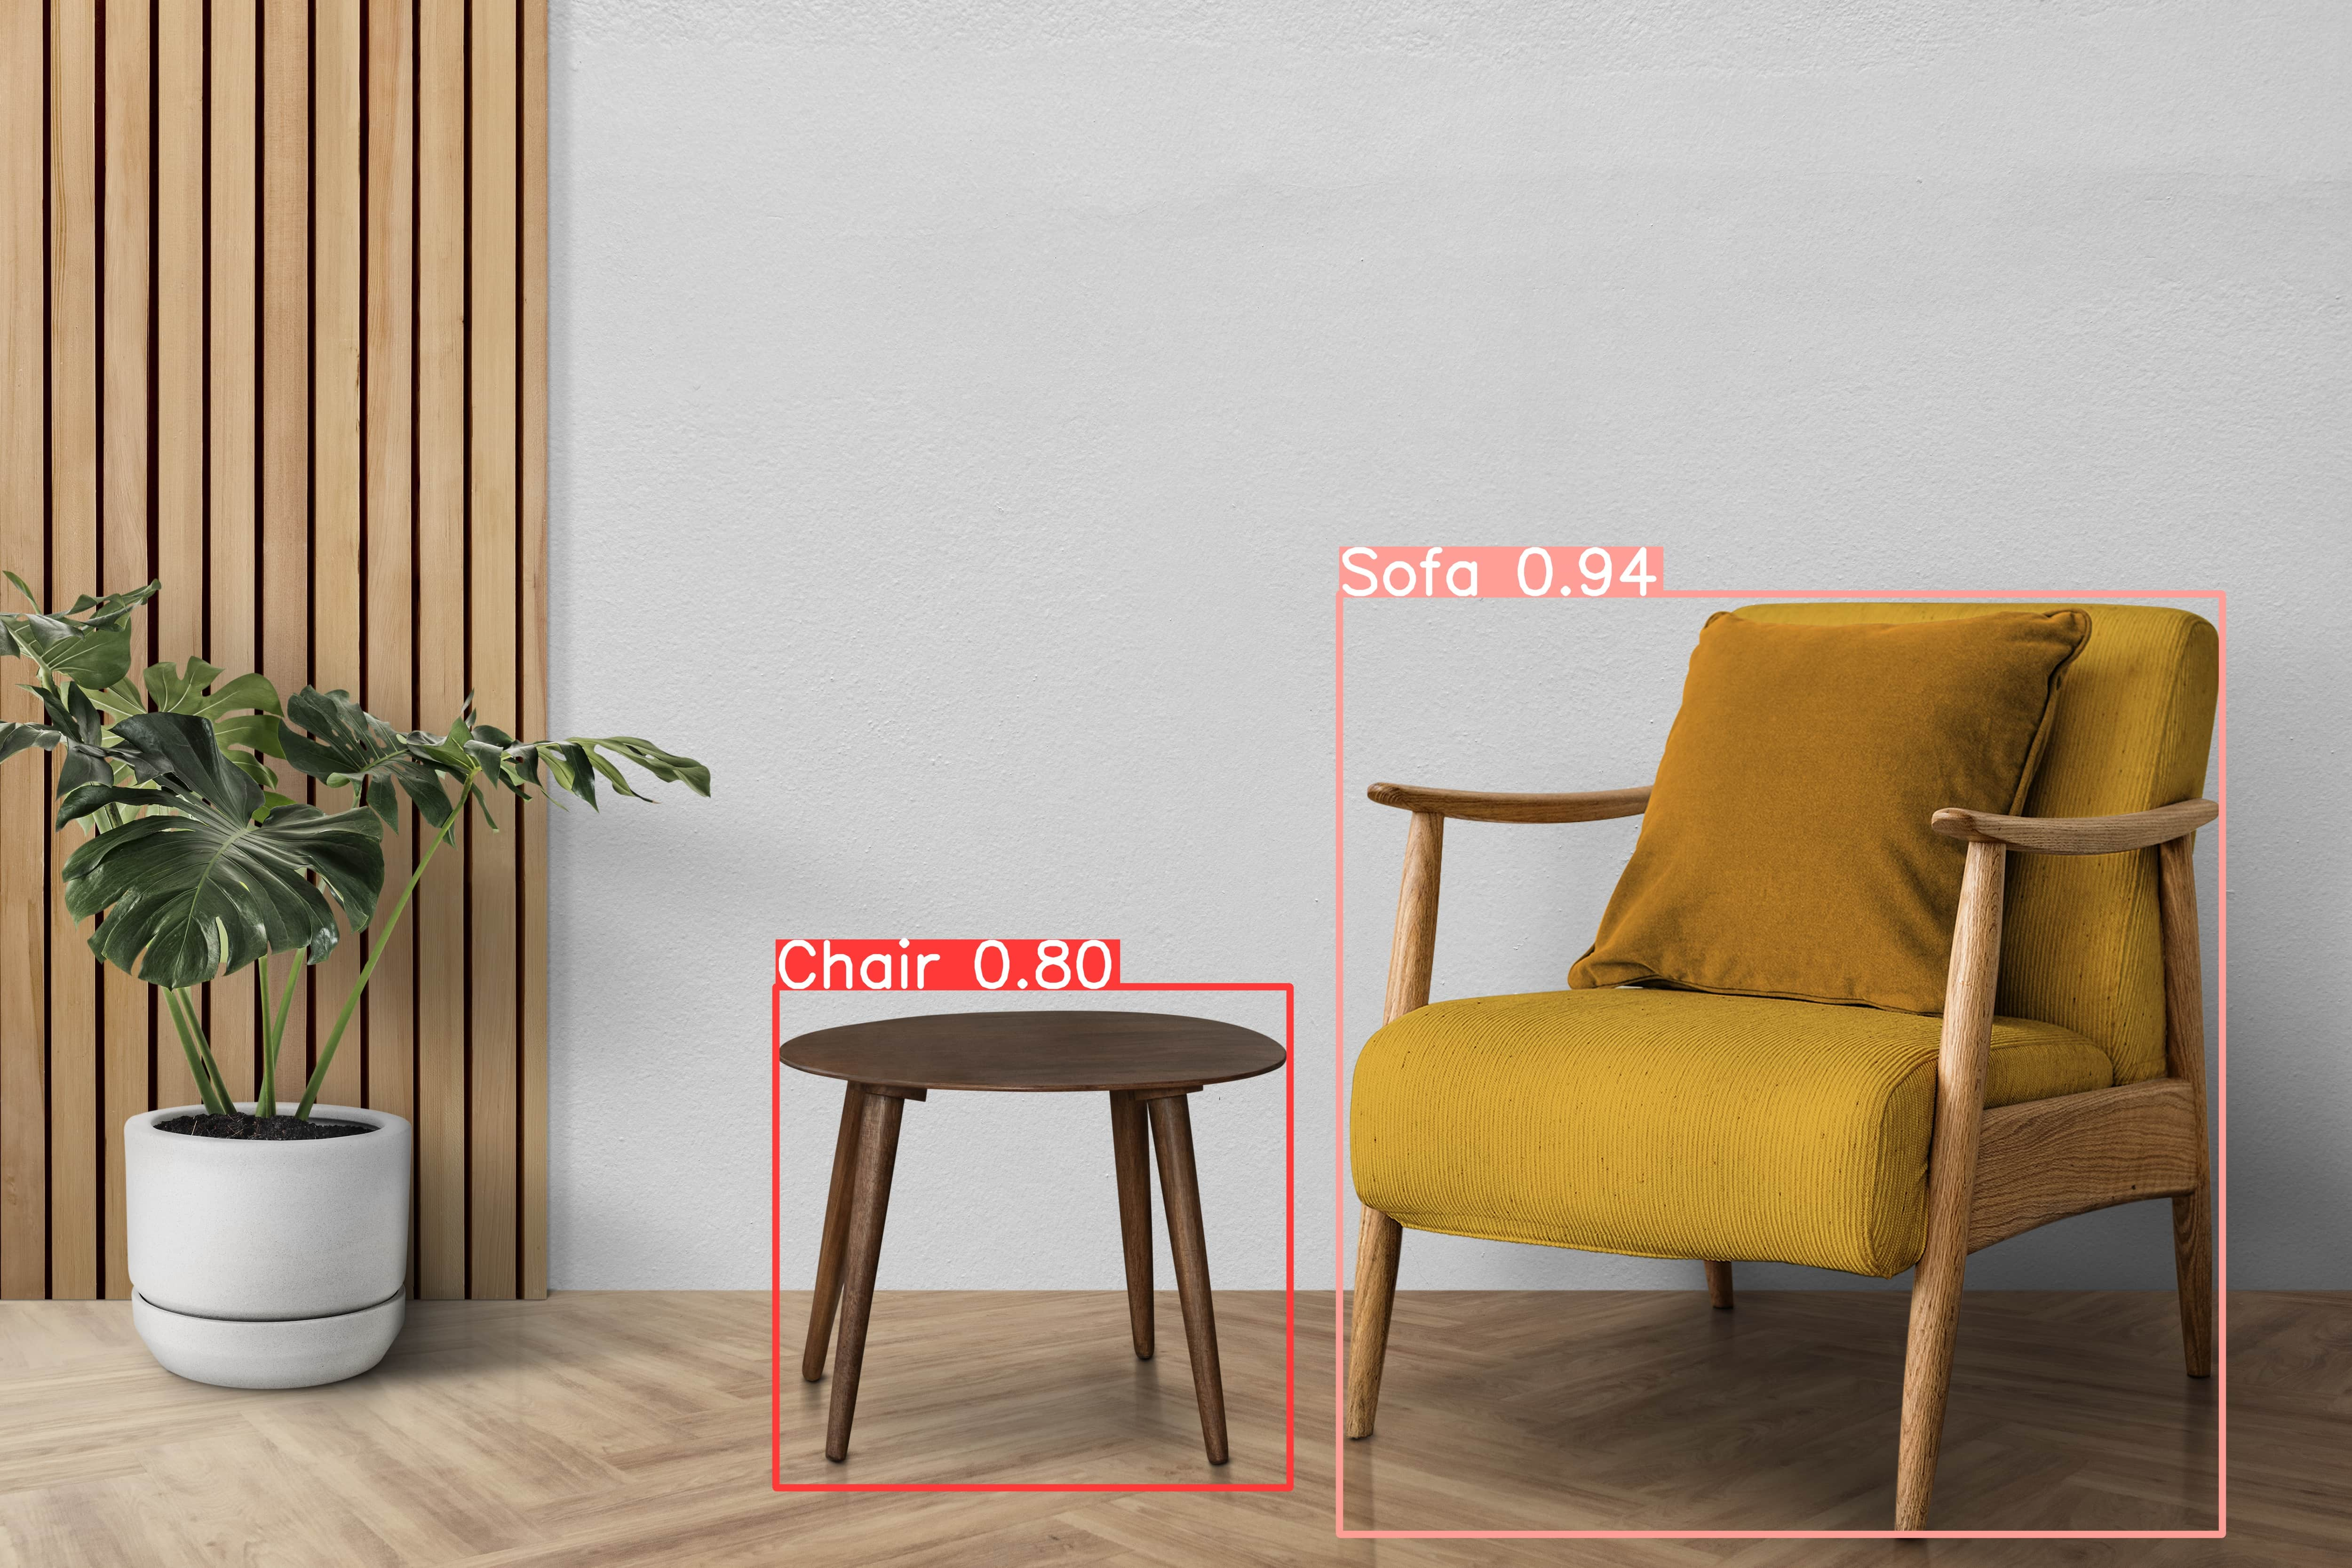
\includegraphics[scale=.08]{img/result.jpg}
\caption{Kết quả dự đoán của mô hình sau khi huấn luyện}
\label{fig:my_label_with_H}
\end{figure}




\section{Mã nguồn và tài liệu tham khảo}
\href{https://colab.research.google.com/drive/1FOSz6e9F2uOTFiB6gteMiklTc6aOFNJY?usp=sharing}{Mã nguồn Colab} \\
\href{https://universe.roboflow.com/minoj-selvaraj/furniture-sfocl.}{Link dataset chính thống} \\
\href{https://linkvertise.com/720390/yolov8-funiture-dataset?o=sharing}{Link dataset đã định dạng theo YOLOv7} \\ 
\href{https://github.com/ultralytics/ultralytics/blob/main/docs/en/models/yolov10.md}{Github YOLOv10} \\
\href{https://arxiv.org/pdf/2405.14458}{Paper YOLOv10}



% References
% \cleardoublepage
\phantomsection
\addcontentsline{toc}{section}{Tài liệu}
\bibliographystyle{plain}
\bibliography{ref/ref}

% % Appendix
% \appendix
% % Add \cleardoublepage to move appendices to next page.
% \section{Phụ lục}
\begin{itemize}
\item Template này \textbf{không phải} là template chính thức của Khoa Công nghệ thông tin - Trường Đại học Khoa học Tự nhiên.
\item Các hình ảnh, bảng biểu, thuật toán trong template chỉ mang tính chất ví dụ.
\item Nhóm tác giả phân phối \textbf{miễn phí} template này \href{https://github.com/khongsomeo/hcmus-unofficial-report-template}{trên GitHub} và \href{https://www.overleaf.com/latex/templates/hcmus-report-template/zyrhmsxynwqs}{trên Overleaf} với \href{https://github.com/khongsomeo/hcmus-unofficial-report-template/blob/main/LICENSE}{Giấy phép GNU General Public License v3.0}. Nhóm tác giả không chịu trách nhiệm với các bản phân phối không nằm trong hai kênh phân phối chính thức nêu trên.
\end{itemize}

\end{document}